\documentclass[a4paper, 11pt]{article}

%%% Packages
\usepackage[margin=50pt, vmargin={50pt, 10pt},includefoot]{geometry}
\usepackage{palatino}

%%% Listing package
\usepackage{listings}
\usepackage{color}
\usepackage{url}
\usepackage{hyperref}
\usepackage{setspace}
\usepackage{graphicx}
\DeclareGraphicsExtensions{.pdf,.png,.jpg}
\hypersetup{
  colorlinks = false,
  pdfborder={0 0 0}
}

\definecolor{dkgreen}{rgb}{0,0.6,0}
\definecolor{gray}{rgb}{0.5,0.5,0.5}
\definecolor{mauve}{rgb}{0.58,0,0.82}
\definecolor{red}{rgb}{0.8,0,0}
\definecolor{dkblue}{rgb}{0,0,0.6}

\lstset{ 
  language=C++,                  % the language of the code
  basicstyle=\footnotesize,       % the size of the fonts that are used for the code
  numbers=left,                   % where to put the line-numbers
  numberstyle=\tiny\color{gray},  % the style that is used for the line-numbers
  stepnumber=1,                   % the step between two line-numbers. If it's 1, each line 
  numbersep=5pt,                  % how far the line-numbers are from the code
  backgroundcolor=\color{white},      % choose the background color. You must add \usepackage{color}
  showspaces=false,               % show spaces adding particular underscores
  showstringspaces=false,         % underline spaces within strings
  showtabs=false,                 % show tabs within strings adding particular underscores
  frame=single,                   % adds a frame around the code
  rulecolor=\color{black},        % if not set, the frame-color 
  captionpos=b,                   % sets the caption-position to bottom
  breaklines=true,                % sets automatic line breaking
  breakatwhitespace=false,        %sets if automatic breaks should only happen at whitespace
  title=\lstname,                   % show the filename of files included with \lstinputlisting;
  keywordstyle=\color{blue},         % keyword style
  keywordstyle=[2]\color{dkgreen},
  commentstyle=\color{red},       %comment style
  keywords=[2]{vector, Action, State},
  stringstyle=\color{mauve},         %string literal style
  escapeinside={\%*}{*)},            % if you want to add LaTeX within your code
  emph={string, Puzzle, Board, multiset},  % emphasized characters
  emphstyle={\color{dkgreen}}
}

%%% End listing

%%%%%%%%%%%%%%%%%%%%%%%%%%%%%%%%%%%%%%%%%%%%%%%%%%%%%%%%%%%%%%%%%%%%%%%%%%%%%%%%%%%%%%%%%%%%%%%%%%%%%%%%%%%%%%%%%%%%%%%%%%%%%%%%%%%%%%%%%%%%%%%%%%%%%%%%%%%%%%%%%%%%%%%%%%%%%% 
\begin{document}
\title{Pattern Informatics Report}
\author{Le Trung Kien\\ 
  03-120291, 3rd Year \\
  Department of Mechano-Informatics \\ 
  The University of Tokyo
}
\maketitle

\section{Widrow-Hoff Algorithm \& Pseudo-Inverse Matrix}
Widrow-Hoff Algorithm based on gradient descent method to update model's weight as following:
\[ W_{new} = W_{old} - \alpha W_{old} (X W_{old} - T)\]
In which, $\alpha$ is learning rate, $W$ is weight, $X$ is training data, $T$ is training label. The training will stop when error reaches a threshold or number of iterations exeeds limit. In my implementation, learning rate is 0.1, threshold is 0.001 and max number of iterations is 100. \\
On the other hand, optimal value can be directly calculated by using pseudo-inverse matrix:
\[ W = (X^{T}X)^{-1}X^TT\]
Results after using the two above algorithms are shown in Figure 1.
\begin{figure}[hbt]
  \centering
  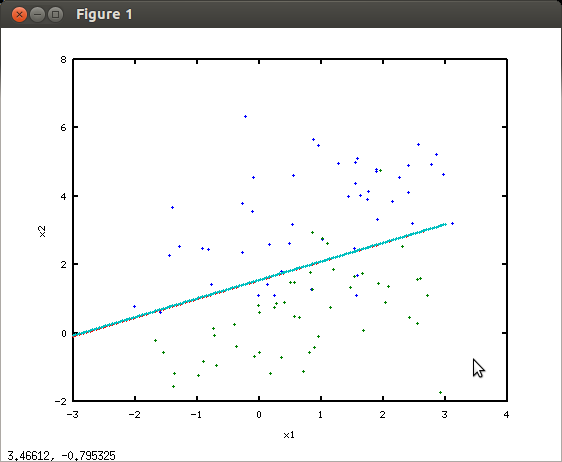
\includegraphics[width=4in]{1-2.png}
  \caption[Close up of \textit{Hemidactylus} sp.]
  {Classification by Widrow-Hoff algorithm and pseudo-inverse matrix.}
\end{figure}

According to Figure 1, the two weights trained by the two algorithms are almost the same, which is not obvious fact. In this case, the two classes are linearly separable, so the two algorithms should lead to very simal final weight. Still, they are slightly different because the weight calculated by pseudo-inverse matrix is deterministic while the one trained by Willow-Hoff depends on numerous factors such as intial values, error's threshold and number of iterations. Moreover, Willow-Hoff algorithm is always a valid method, but when pseudo-inverse matrix of $X$ does not exist, we cannot use it to find the optimal weight for classification. \\

An example of running the program (Willow-Hoff and Pseudo-Inverse in order):
\begin{verbatim}
@:~/Pattern$ ./2 1
0.642855
0.223755
-0.412262
Precision's rate: 0.875
@:~/Pattern$ ./2 2
0.644933
0.223556
-0.412747
Precision's rate: 0.875
\end{verbatim}

\section{Leave-one-out Method}

\section{Mahalanobis Distance}
\end{document}
%%%%%%%%%%%%%%%%%%%%%%%%%%%%%%%%%%%%%%%%%%%%%%%%%%%%%%%%%%%%%%%%%%%%%%%%%%%%%%%%%%%%%%%%%%%%%%%%%%%%%%%%%%%%%%%%%%%%%%%%%%%%%%%%%%%%%%%%%%%%%%%%%%%%%%%%%%%%%%%%%%%%%%%%%%%%%%
